\section{Introduction to Proofs}

\frame{
{Part 1: Introduction to Proofs.}

\tableofcontents[currentsection,hideallsubsections, firstsection=2, sections={2-4}]
}

\subsection{What is a Proof?}

\begin{frame}{What is a proof?}

  Some concepts are easy to understand, but not easy to show that they are true.\bigskip

  \begin{columns}
    \column{0.3\textwidth}
      \centering
      \includegraphics[width=.5\textwidth]{../img/triangle_rect}
    \column{0.7\textwidth}
      \begin{itemize}
        \item Pythagoras Theorem:
        \begin{equation*}
          a^2+b^2=c^2
        \end{equation*}
        \item It is easy to show this is true for {\bf any one triangle}.
        \item But how do you show it is is true for {\bf all} triangles?
      \end{itemize}
  \end{columns}
  \bigskip

  The proof of the Pythagoras theorem is {not obvious}: there are more than 100 different proofs!
\end{frame}

\begin{frame}{What is a proof?}{One Pythagoras Proof}

  \begin{columns}[T]
    \column{0.7\textwidth}
      \begin{itemize}
        \item {\bf Proof}: by geometric construction
        \item Arrange four identical triangles;
        \item Show that internal angles are right;
        \item Internal square area: $c^2$
        \item External square area: $(a+b)^2$
        \item $(a+b)^2 = c^2 + 4(\text{area triangle})$
        \item $(a+b)^2 = c^2 + 4(\frac{ab}{2})$
        \item $a^2 + 2ab + b^2 = c^2 + 2ab$
        \item $a^2 + b^2 = c^2$ \hfill $\blacksquare$
      \end{itemize}
    \column{0.3\textwidth}
      \includegraphics[width=\textwidth]{../img/triangle_pytagoras}
  \end{columns}
  \bigskip

  The {\bf Key Idea} of this proof is that $a$, $b$ and $c$ can be assigned to \alert{any right triangle}.\\
  But how do we find a new proof?
\end{frame}

\begin{frame}{False Proofs -- Infinite Chocolate!}
  \begin{block}{}
    \begin{itemize}
      \item \alert{Be Careful!} -- It can be very hard to detect a wrong step in a proof.
      \item A wrong proof can be used to say something impossible is true.
      \item What is wrong in the proof below? \only<2>{\alert{Always check your assumptions!}}
    \end{itemize}
  \end{block}

  \begin{center}
    \includegraphics[width=.9\textwidth]{../img/false_proof}
  \end{center}
\end{frame}

\subsection{Proofs and Computer Science}

\begin{frame}[t]{Proofs and Computer Science}

  \begin{center}
    {\bf Why are proofs important for Computer Science?}
  \end{center}
  \bigskip

  \begin{itemize}
    \item Proofs can be used {\bf to show that a program is correct}.\\
    (or to show that a program is incorrect)
  \end{itemize}

  \vfill

  \begin{block}{Examples}
    \begin{itemize}
      \item Prove that the output of a program is correct for any input.
      \item Prove that certain input will cause a bug or crash in a program.
      \item Prove that a program finishes in $N$ steps;
    \end{itemize}
  \end{block}


\end{frame}

\begin{frame}[fragile]{Proofs and Computer Science}{Example:}

  Can you prove that the program below is correct (or incorrect)?

  \begin{itemize}
    \item To prove correctness, must prove for {\bf any} input $a,b,c$
    \item To prove incorrectness, it is enough to show {\bf one} input
  \end{itemize}

\begin{verbatim}
int triangle_type(int a, int b, int c)
  // a, b, c are the length of the sides of a triangle;
  if (a == b)
    if (b == c)        return "all sides are equal";
    else               return "two sides are equal";
  else if (b == c)     return "two sides are equal";
  else                 return "all sides are different";
\end{verbatim}
\end{frame}

\begin{frame}[t]{Proof Methods}{}
  How do we prove something?
  \begin{block}{}
    For every nonnegative integer $n$, the value of $n^2+n+41$ is prime.
  \end{block}\medskip

  We could try to test values of $n$ one by one:
  \begin{center}
    $n = 0; n^2+n+41 = 41$, prime; $n = 1; n^2 + n + 41 = 43$, prime; $n = 2; 47$, prime; $\ldots$, $n = 20; 461$, prime...
  \end{center}\medskip

  \begin{itemize}
    \item When do we stop?
    \item ($n = 40; 41\times41$, is not prime...)
  \end{itemize}\bigskip

  We need better ways to prove things!
\end{frame}